\section{Robot characteristics}\insertloftspace
\setcounter{figure}{0}\setcounter{table}{0}

In parallel to the design, we simulated the operation of the robot using Matlab, Simulink and python. The work explained from now on is done on the last prototype presented in the previous section. However, the principle applied has been the same throughout the project. The simultaneous work was important in order to anticipate the delays due to the manufacturing of the robot. 

\subsection{Kinematics}

\textbf{Definition :} Given a vector $x=[x_1 x_2 x_3]^T \in \mathbb{R}^3$, we define : 
\begin{center}
    $[x] = \begin{bmatrix}
        0 & -x_3 & x_2 \\
        x_3 & 0 & -x_1 \\
        -x_2 & x_1 & 0 \\
    \end{bmatrix}$
\end{center}

\noindent\textbf{Definition :} Given two vectors $x$ and $y$ in $\mathbb{R}^3$, we define : $x\times y = [x]\cdot y$

\bigbreak
\noindent\textbf{Definition :} For a joint, we define the pitch $h = \frac{v}{w}$ with v : the linear speed and w the angular speed

\bigbreak
\noindent\textbf{Definition :} The screw is a $6\times1$ vector that represent the angular velocity when $\dot{\theta}=1$ and the linear velocity of the origin when $\dot{\theta}=1$. $S = \begin{bmatrix} s_w\\s_v\end{bmatrix}$ with $s_v = hw-s_w\times q$ where h is the pitch and q is a point on the 

\noindent\textbf{Definition :} For a given reference frame, a screw axis S is written as 
\begin{center}
    $S=\begin{bmatrix}
        s_w\\s_v
    \end{bmatrix}$
\end{center}
where either (i) $\|s_w\|$ = 1 or (ii) $\|s_w\|$ = 0 and $\|s_v\|$ = 1. If the pitch is finite ($h$ = 0 for a pure rotation), then $s_v = hs_w-s_w\times q$ where q is a point on the axis of the screw

\bigbreak
The figure below shows the kinematics schema of the robot. The figure defines an \{s\} frame at the bottom, an \{e\} frame at the end effector position and a \{c\} frame at the camera position. The robot is at is home configuration. The joint are represented with the rotation (positive rotation about the axes is by the right hand rule).

\bigbreak 
The parameters can be found with Onshape and are listed below: 

\begin{center}
    \fcolorbox{black}{white}{
        \begin{minipage}{0.8\linewidth}
            $L_0 = 0.069m$ \hspace{3cm} $d_0 = 0m$ \hfill $h_0 = 0.06m$ \\
            $L_1 = 0.116m$ \hspace{3cm} $d_1 = 0.018m$ \\ 
            $L_2 = 0.16m$ \hspace{3.2cm} $d_2 = 0.042m$ \\ 
            $L_3 = 0.155m$ \hspace{3cm} $d_3 = 0.01413m$ \\ 
            $L_c = 0.053m$ \hspace{3cm} $d_c = 0.0105m$ \hfill $h_c = 0.0815m$ \\
            $L_e = 0.2377m$ \hfill $d_e = 0.0105$ \hfill $h_e = 5.10^{-5}m$ \\
        \end{minipage}
    }
\end{center}

\begin{figure}[ht]
    \centering
    \includegraphics[width=0.8\textwidth]{images/Section04/kinematics\_schema.png}
    \caption{Kinematics schema}
    \label{fig:mesh10}
\end{figure}
\FloatBarrier

\bigbreak
We can then define $M_c$ and the $M_e$ the transformation matrix ($T_{sc}$ and $T_{se}$) when the robot is at its home configuration. 

\bigbreak
\begin{center}
    $
    M_c = \begin{bmatrix}
        0 & 0 & 1 & -h_0-L_3-h_c\\
        0 & -1 & 0 & d_1-d_2+d_3+d_c\\
        1 & 0 & 0 & l_0+l_1+l_2+l_c\\
        0 & 0 & 0 & 1
    \end{bmatrix}
    $
    and
    $
    M_e = \begin{bmatrix}
        0 & 0 & 1 & -h_0-L_3-h_c\\
        0 & -1 & 0 & d_1-d_2+d_3+d_c\\
        1 & 0 & 0 & l_0+l_1+l_2+l_c\\
        0 & 0 & 0 & 1
    \end{bmatrix}
    $
\end{center}

\subsubsection{Base frame}

In this subsection we study the kinematics parameters in the base frame \{s\}. It will be the one used in the followings sections.

\bigbreak
The rotation axis $S_{w_i}$ of each joint  in \{s\} are : 
\begin{center}
    $S_{w_1} = \begin{bmatrix} 0 \\ 0 \\ -1\end{bmatrix}$,
    $S_{w_2} = \begin{bmatrix} 0 \\ 1 \\ 0\end{bmatrix}$,
    $S_{w_3} = \begin{bmatrix} 0 \\ -1 \\ 0\end{bmatrix}$,
    $S_{w_4} = \begin{bmatrix} 0 \\ -1 \\ 0\end{bmatrix}$,
\end{center}

\bigbreak
We can also write the position of each joint  $q_1,q_2,q_3,q_4,q_c,q_e$ in \{s\}. Lining up the position as columns, we get : 

\begin{center}
    $
    \begin{bmatrix}
        -h_0 & -h_0 & -h_0 & -h_0-L_3 & -h_0-L_3-h_c & -h_0-L_3-L_e  \\
        0 & d_1 & d_1-d_2 & d_1-d_2+d_3 & d_1-d_2+d_3+d_c & d_1-d_2+d_3+d_e \\
        L_0 & L_0+L_1 & L_0+L_1+L_2 & L_0+L_1+L_2 & L_0+L_1+L_2+L_c & L_0+L_1+L_2+h_e \\
    \end{bmatrix}
    $
\end{center}

\bigbreak
There are all pure rotation joint, using the position, the rotation axis and the formula define in above we can calculate the screw axis $S_1,S_2,S_3,S_4$ in \{s\}.. Lining up them as columns, we get : 

\begin{center}
    $S_{list} = 
    \begin{bmatrix}
        0 & 0 & 0 & 0 \\
        0 & 1 & -1 & -1 \\
        -1 & 0 & 0 & 0 \\
        0 & -L_0-L_1 & L_0+L_1+L_2 & L_0+L_1+L_2 \\
        -h_0 & 0 & 0 & 0 \\
        0 & -h_0 & h_0 & h_0+L_3
    \end{bmatrix}
    $
\end{center}

\subsubsection{End effector frame}

In this subsection we study the kinematics parameters in the end effector frame \{e\}. However, it is not the one that will be use later. 

\bigbreak
The rotation axis $S_{w_i}$ of each joint  in \{e\} are : 
\begin{center}
    $S_{w_1} = \begin{bmatrix} -1 \\ 0 \\ 0\end{bmatrix}$,
    $S_{w_2} = \begin{bmatrix} 0 \\ -1 \\ 0\end{bmatrix}$,
    $S_{w_3} = \begin{bmatrix} 0 \\ 1 \\ 0\end{bmatrix}$,
    $S_{w_4} = \begin{bmatrix} 0 \\ 1 \\ 0\end{bmatrix}$,
\end{center}

\bigbreak
We can also write the position of each joint  $q_1,q_2,q_3,q_4,q_c,q_e$ in \{e\}. Lining up the position as columns, we get : 

\begin{center}
    $
    \begin{bmatrix}
        -h_e-L_2-L_1 & -h_e-L_2 & -h_e & -h_e & -h_e+L_c & 0  \\
        d_e+d_3-d_2+d_1 & d_e+d_3-d_2 & d_e+d_3 & d_e & d_e-d_c & 0 \\
        L_e+L_3 & L_e+L_3 & L_e+L_3 & L_e & L_e-h_c & 0 \\
    \end{bmatrix}
    $
\end{center}

\bigbreak
There are all pure rotation joint, using the position, the rotation axis and the formula define in above we can calculate the screw axis $B_1,B_2,B_3,B_4$ in \{e\}.. Lining up them as columns, we get : 

\begin{center}
    $B_{list} = 
    \begin{bmatrix}
        -1 & 0 & 0 & 0 \\
        0 & -1 & 1 & 1 \\
        -1 & 0 & 0 & 0 \\
        0 & L_e+L_3 & -L_e-L_3 & -L_e \\
        -L_e-L_3 & 0 & 0 & 0 \\
        d_e+d_3-d_2+d_1 & h_e+L_2 & -h_e & -h_e
    \end{bmatrix}
    $
\end{center}

\subsection{Workspace}

In order to define our robot, we have determined the workspace. To do this, we used the forward kinematic computed with python as explained in section 5. Knowing the limits of each link, we made loops to evaluate the reachable positions in the whole space. We then represented the working space according to the 3 planes of the robot: top, front and side. Obviously, this does not allow to visualize the complete workspace, but it is the clearest way to show it. However, our calculations allow us to access the complete workspace, i.e. all the points reachable by the robot. We also put the python code to represent these figures. The robot is also present on the figures in red in its zero confugration to better estimate the working space.

\begin{figure}[ht]
    \centering
    \includegraphics[width=0.8\textwidth]{images/Section04/workspace\_xy\_plan.png}
    \caption{Workspace in xy plan for z=0.07m}
    \label{fig:mesh22}
\end{figure}
\FloatBarrier

\begin{figure}[ht]
    \centering
    \includegraphics[width=0.8\textwidth]{images/Section04/workspace\_xz\_plan.png}
    \caption{Workspace in xz plan for y=0m}
    \label{fig:mesh23}
\end{figure}
\FloatBarrier

\begin{figure}[ht]
    \centering
    \includegraphics[width=0.8\textwidth]{images/Section04/workspace\_yz\_plan.png}
    \caption{Workspace in yz plan for x=-0.06m }
    \label{fig:mesh24}
\end{figure}
\FloatBarrier

\begin{minted}[linenos=true,bgcolor=LightYellow]{Python}
    # import kinematics parameters
    from parameters import * 
    import matplotlib.pyplot as plt
    # joint values in radian
    pelvis_limits = list(np.arange(-1.57,1.57,0.2))
    shoulder_limits = list(np.arange(-1.57,0.69,0.3))
    elbow_limits = list(np.arange(-1.57,1.05,0.4))
    wrist_limits = list(np.arange(0,1.57,0.4))
    # loop on values to get all positions
    x,y,z = [],[],[]
    for pelvis in pelvis_limits:
        for shoulder in shoulder_limits:
            for elbow in elbow_limits:
                for wrist in wrist_limits:
                    thetalist = np.array([pelvis,shoulder,elbow,wrist])
                    # compute transformation matrix and point
                    t = mr.FKinSpace(m_e,screw_list,thetalist)
                    p = t.dot(np.array([0,0,0,1]))[:-1]
                    x.append(p[0])
                    y.append(p[1])
                    z.append(p[2])
    # plot xy plan
    plt.axes()
    plt.plot(x,y,".b",ms = 3,alpha=0.3) # plot position
    plt.plot([p1[0],p2[0],pe[0]], [p1[1],0,pe[1]],"-r") # plot robot arm
    rectangle = plt.Rectangle((-0.12,-0.06), 0.24, 0.12, fc='red',ec="red") 
    plt.gca().add_patch(rectangle) # plot robot body
    plt.title('xy plan')
    plt.xlabel('x (m)')
    plt.ylabel('y (m)')
    \end{minted}

\subsection{Payload}

Another important characteristic of our robot is the payload. This is the maximum mass that can be lifted by our robot before breaking. A cherry tomato weighs on average 15g, so we need a robot able to lift at least 2 times that to avoid any problem. To measure the payload, we placed the robot in the "worst" configuration: arm stretched flat. We then measured the intensity of the shoulder motor to lift a given mass. Then we held the robot in position by blocking it and we operated the same motor by measuring the current at the moment of the break. For a DC motor the current is proportional to the torque which is proportional to the mass, it is then possible to determine the maximum mass that the robot can support. 
\begin{figure}[ht]
    \centering
    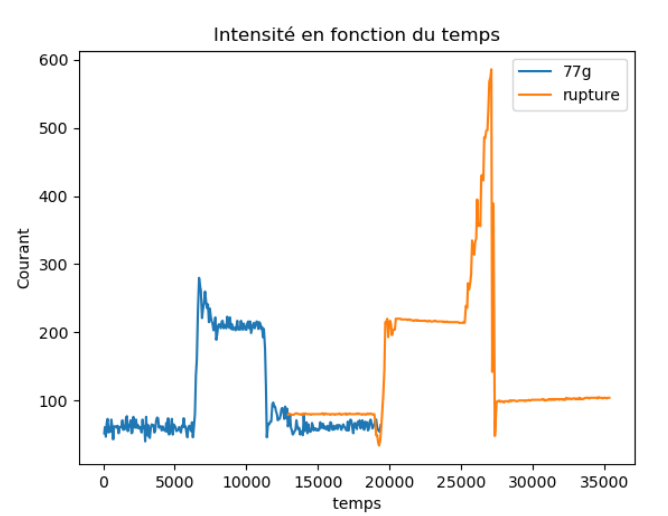
\includegraphics[width=0.8\textwidth]{images/Section04/payload.png}
    \caption{Payload mesure}
    \label{fig:mesh25}
\end{figure}
\FloatBarrier

The graph below shows the intensity in a specific unit of the motor. We measured an intensity of 300 for a mass of 77g and an intensity of 600 at breakage. Thus, \textbf{the payload of our robot is 144g}. We can note that this is not the limit of the robot. Indeed, it is the pvc gear that broke and not the physical limits of the robot. A stronger gear would allow to increase the maximum mass if needed.

\subsection{Precision}

Finally, we have determined the accuracy of our robot. For this, we subjected our robot to a movement of 10cm from left to right several times. We made sure to mark the trajectory of our robot and we measured the real distance covered. It was 12cm on average which makes a \textbf{accuracy of 2cm}. However, as we will see later, this is sufficient with the control method we have selected because the error is naturally compensated by the user.
\begin{figure}[ht]
    \centering
    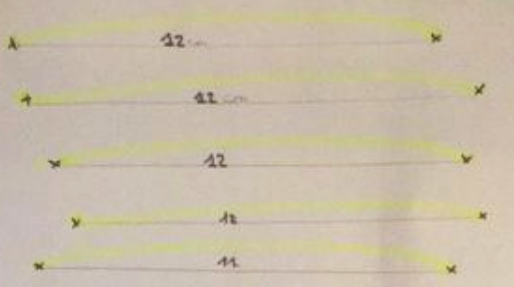
\includegraphics[width=0.8\textwidth]{images/Section04/precision.png}
    \caption{Precision}
    \label{fig:mesh26}
\end{figure}
\FloatBarrier

\subsection{Others}

We also have other characteristics that we have measured:
\begin{itemize}[noitemsep]
    \item height : 70cm including 50cm of arms
    \item mass: 2.7kg of which for 1.2kg the base
\end{itemize}
